%!TEX program = lualatex
\documentclass[aspectratio=169,handout]{beamer}
% add 'handout' to beamer options for printout

\usepackage{multimedia}
\usepackage[backend=biber,style=ieee]{biblatex}

\usetheme{AVThesis}

\title{The Art of Robotics:\\\vspace{0.2em}\huge{Toward a Holistic Approach}}
\subtitle{Master of Science in Robotics\\Thesis Defense}
\author{Alexander Volkov Jr.}
\date{July 31, 2018}

\bibliography{refs/thesis-slides.bib}

% Change frame margins
\addtobeamertemplate{frametitle}{\vspace*{1cm}}{\vspace*{0cm}}

\setcounter{showSlideNumbers}{1}

\begin{document}
	\setcounter{showProgressBar}{0}
	\setcounter{showSlideNumbers}{0}

	\frame{\titlepage}

	\begin{frame}
		\frametitle{Talk Agenda}
		\begin{enumerate}
			\setlength{\itemsep}{4mm}
			\item Background
				\textcolor{AVThesisGrey}{\footnotesize\hspace{1em} The BFD; how I ended up here}
				
%			\item Other Things
%				\textcolor{AVThesisGrey}{\footnotesize\hspace{1em} Warm up the crowd with a quick review of some other things I've done.}
			
			\item The Big Picture
				\textcolor{AVThesisGrey}{\footnotesize\hspace{1em} Cover the central themes of this talk.}
			
			\item A Unifying Framework
				\textcolor{AVThesisGrey}{\footnotesize\hspace{1em} An old framework, revived.}
			
%			\item Brushless PMSM Motors
%				\textcolor{AVThesisGrey}{\footnotesize\hspace{1em} Operating limits, thermal management, liquid cooling.}
	
%			\item Touching Robots
%				\textcolor{AVThesisGrey}{\footnotesize\hspace{1em} Tactile sensing, contact modeling, whiskers, robot pain.}
%			
			\item Conclusions
				\textcolor{AVThesisGrey}{\footnotesize\hspace{1em} Review key points and propose some future work.}
			
			\item Acknowledgments \& Questions
				\textcolor{AVThesisGrey}{\footnotesize\hspace{1em} \emph{``Please clap...''}}
		\end{enumerate}
	\end{frame}

	\setcounter{framenumber}{0}
	\setcounter{showProgressBar}{1}
	\setcounter{showSlideNumbers}{1}
	
	\section{Background}
		
		\begin{frame}
			\frametitle{The BFD}
			\begin{itemize}
				\item \textbf{End Game:} Develop a Unified Framework for Understanding Robotics \pause
				\begin{itemize}
					\item \textbf{Thesis Purpose:} Reflect on and organize \emph{my} understanding of robotics \pause
						\begin{itemize}
							\item \textbf{Talk Purpose:} Provide an overview of my thesis dissertation for the committee
						\end{itemize}
				\end{itemize}
			\end{itemize}
		\end{frame}
		
		\begin{frame}
			\frametitle{Talk Title Etymology I}
			\begin{tikzpicture}[overlay, remember picture]
				\node[anchor=east] (taoe) at ($(current page.east)+(-3mm,-1mm)$) 	{
\includegraphics[width=5.5cm]{media/the-art-of-electronics.png}};
			\end{tikzpicture}
			\begin{itemize}
				\item ``The Art of Electronics'', by \emph{Horowitz \& Hill}\pause
				\begin{itemize}
					\item Literally the electrical engineering bible
					\item Incredibly thorough
					\item Perfect balance of practicality and rigor 
				\end{itemize}
			\end{itemize}
		\end{frame}
	
		\begin{frame}
			\frametitle{Talk Title Etymology II}
			\begin{tikzpicture}[overlay, remember picture]
				\node[anchor=east] (taoe) at ($(current page.east)+(-10mm,-1mm)$) 	{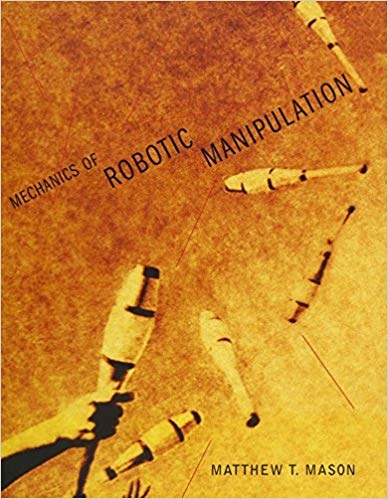
\includegraphics[width=4cm]{media/mason-manip-book.jpg}};
			\end{tikzpicture}
			\begin{itemize}
				\item ``Mechanics of Robotic Manipulation'', by \emph{Mason}\footnotemark~\autocite{mason2001mechanics} \pause
					\begin{itemize}
						\item ``Manipulation is an art\dots'' (p.1)
					\end{itemize}
			\end{itemize}
			\footnotetext{Matt, I'll take my referral payments by mail.}
		\end{frame}

%		\begin{frame}
%			\frametitle{Talk (Sub)Title Etymology III}
%			\begin{tikzpicture}[overlay, remember picture]
%			\fontsize{18}{15}
%			\node[anchor=center] (subtitle) at (current page.center) {``Toward a Holistic Approach''};
%			\end{tikzpicture}
%		\end{frame}
%		
%		\begin{frame}
%			\addtocounter{framenumber}{-1}
%			\frametitle{Talk (Sub)Title Etymology III}
%			\begin{tikzpicture}[overlay, remember picture]
%				\fontsize{18}{15}
%				\node[anchor=center] (subtitle) at (current page.center) {``\highlight{toward}{Toward} a Holistic Approach''};
%				\fontsize{10}{12}
%				\node[anchor=south west, fill=red!20,rounded corners, text width=3cm, outer sep=3pt, inner sep=3pt] (toward-note) at ($(current page.south west) + (10mm,10mm)$) {When you concede falling short of a goal in academia.};
%				\draw [->, line width=0.3mm] (toward-note) -- (toward);
%			\end{tikzpicture}
%		\end{frame}
	
		\begin{frame}
%			\addtocounter{framenumber}{-1}
			\frametitle{Talk (Sub)Title Etymology III}
			\begin{tikzpicture}[overlay, remember picture]
				\fontsize{18}{15}
				\only<1>{\node[anchor=center] (subtitle) at (current page.center) {``Toward a Holistic Approach''};}
				\only<2>{\node[anchor=center] (subtitle) at (current page.center) {``\highlight{toward}{Toward} a Holistic Approach''};
				\fontsize{10}{12}
				\node[anchor=south west, fill=red!20,rounded corners, text width=5cm, outer sep=3pt, inner sep=3pt] (toward-note) at ($(current page.south west) + (10mm,10mm)$) {When you concede falling short of a goal in academia. Example: Mason's Annual Review ``Toward Robotic Manipulation'' \autocite{Mason2018}};
				\draw [->, line width=0.3mm] (toward-note) -- (toward);}
				\onslide<3->{\node[anchor=center] (subtitle) at (current page.center) {``\highlight{toward}{Toward} a \highlight{holistic}{Holistic} Approach''};
				\fontsize{10}{12}
				\node[anchor=south west, fill=red!20,rounded corners, text width=5cm, outer sep=3pt, inner sep=3pt] (toward-note) at ($(current page.south west) + (10mm,10mm)$) {When you concede falling short of a goal in academia. Example: Mason's Annual Review ``Toward Robotic Manipulation'' \autocite{Mason2018}};
				\draw [->, line width=0.3mm] (toward-note) -- (toward);
				\node[anchor=south east, fill=red!20,rounded corners, text width=7cm, outer sep=3pt, inner sep=3pt] (holistic-note) at ($(current page.south east) + (-10mm,10mm)$) {From the mechatronics/systems engineering community. Chhabra and Emami provide an excellent summary in \autocite{Chhabra2011}.};
				\draw [->, line width=0.3mm] (holistic-note) -- (holistic);}
			\end{tikzpicture}
		\end{frame}

	
		\begin{frame}
			\frametitle{How I Ended Up Here (Some Context) I}
			\vspace{-0.5em}
			\begin{itemize}
				\item \textbf{Hobby robotics} $\Rightarrow$ self-taught basic electronics, programming, CAD\pause
					\begin{itemize}
						\item ``Keep it cheap''
						\item ``Keep it open-source''
						\item ``Keep it useful (or, at least, artistic)''
					\end{itemize}\pause
				\vspace{0.5em}
				\item \textbf{Cornell Undergrad} $\Rightarrow$ ECE major, ME/CS minors\pause
					\begin{itemize}
						\item \textbf{ECE:}
							\begin{itemize}
								\item ``Everything is an impedance (or an admittance)''
								\item ``What's the system bandwidth?''
							\end{itemize}
						\item \textbf{ME:}\pause
							\begin{itemize}
								\item ``At the end of the day, everything is mechanical''
								\item ``Everything is a model, and every model is wrong''
							\end{itemize}\pause
						\item \textbf{CS:} 
						\begin{itemize}
							\item ``90\% of solving a problem is finding the right representation''
							\item ``Everything breaks at the interfaces''
						\end{itemize}
					\end{itemize}
			\end{itemize}
		\end{frame}
	
		\begin{frame}
			\addtocounter{framenumber}{-1}
			\frametitle{How I Ended Up Here (Some Context) II}
			\begin{tikzpicture}[overlay, remember picture]
				\node[anchor=center] (ri-logo) at (current page.center) {
\includegraphics[width=30mm]{assets/ri-logo.eps}};
				\node[minimum width=2cm, below=5mm of ri-logo] {``Time to become a robotics master...''};
			\end{tikzpicture}
		\end{frame}
	
		\begin{frame}
			\addtocounter{framenumber}{-1}
			\frametitle{How I Ended Up Here (Some Context) III}
			\begin{tikzpicture}[overlay, remember picture]
				\node[anchor=south east] (ri-logo) at ($(current page.south east)+(-5mm,10mm)$) {
\includegraphics[width=16mm]{assets/ri-logo.eps}};
				\fontsize{12}{10}
				\node[anchor=south west] (me) at ($(current page.south west)+(5mm,10mm)$) {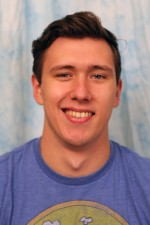
\includegraphics[width=2cm]{media/me.jpg}};
				\node[minimum width=2cm, right=3mm of me] {``Legged locomotion is cool...''};
			\end{tikzpicture}
		\end{frame}

		\begin{frame}
			\addtocounter{framenumber}{-1}
			\frametitle{How I Ended Up Here (Some Context) IV}
			\begin{tikzpicture}[overlay, remember picture]
				\node[anchor=south east] (ri-logo) at ($(current page.south east)+(-5mm,10mm)$) {
\includegraphics[width=16mm]{assets/ri-logo.eps}};
				\fontsize{12}{10}
				\node[anchor=south west] (me) at ($(current page.south west)+(5mm,10mm)$) {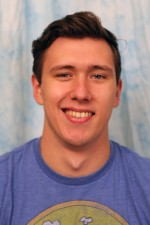
\includegraphics[width=2cm]{media/me.jpg}};
				\node[minimum width=2cm, right=3mm of me] {\color{gray}``Legged locomotion is cool...''};
				\node[anchor=north east] (hartmut) at ($(current page.north east)+(-5mm,-15mm)$) {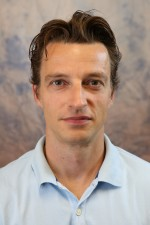
\includegraphics[width=2cm]{media/hartmut.jpg}};
				\node[anchor=north east] (travers) at ($(current page.north east)+(-28mm,-15mm)$) {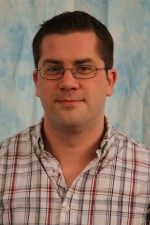
\includegraphics[width=2cm]{media/travers.jpg}};
				\node[anchor=north east] (koushil) at ($(current page.north east)+(-51mm,-15mm)$) {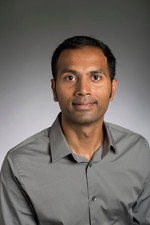
\includegraphics[width=2cm]{media/koushil.jpg}};
				\node[anchor=east, minimum width=2cm, left=3mm of koushil] {``Great! Here's absolutely no funding.''};
			\end{tikzpicture}
		\end{frame}
	
		\begin{frame}
			\addtocounter{framenumber}{-1}
			\frametitle{How I Ended Up Here (Some Context) V}
			\begin{tikzpicture}[overlay, remember picture]
				\node[anchor=south east] (ri-logo) at ($(current page.south east)+(-5mm,10mm)$) {
\includegraphics[width=16mm]{assets/ri-logo.eps}};
				\fontsize{12}{10}
				\node[anchor=south west] (me) at ($(current page.south west)+(5mm,10mm)$) {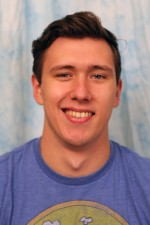
\includegraphics[width=2cm]{media/me.jpg}};
				\node[minimum width=2cm, right=3mm of me] {``Umm...''};
				\node[anchor=north east] (hartmut) at ($(current page.north east)+(-5mm,-15mm)$) {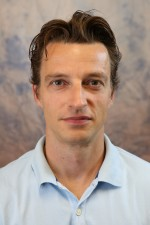
\includegraphics[width=2cm]{media/hartmut.jpg}};
				\node[anchor=north east] (travers) at ($(current page.north east)+(-28mm,-15mm)$) {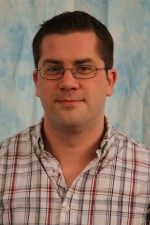
\includegraphics[width=2cm]{media/travers.jpg}};
				\node[anchor=north east] (koushil) at ($(current page.north east)+(-51mm,-15mm)$) {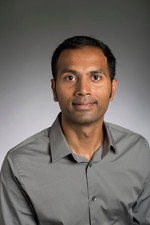
\includegraphics[width=2cm]{media/koushil.jpg}};
				\node[anchor=east, minimum width=2cm, left=3mm of koushil] {\color{gray}``Great! Here's absolutely no funding.''};
			\end{tikzpicture}
		\end{frame}
	
		\begin{frame}
			\addtocounter{framenumber}{-1}
			\frametitle{How I Ended Up Here (Some Context) VI}
			\begin{tikzpicture}[overlay, remember picture]
				\node[anchor=south east] (ri-logo) at ($(current page.south east)+(-5mm,10mm)$) {
\includegraphics[width=16mm]{assets/ri-logo.eps}};
				\fontsize{12}{10}
				\node[anchor=south west] (me) at ($(current page.south west)+(5mm,10mm)$) {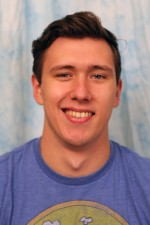
\includegraphics[width=2cm]{media/me.jpg}};
				\node[minimum width=2cm, right=3mm of me] {\color{gray}``Umm...''};
				\node[anchor=north east] (ross) at ($(current page.north east)+(-5mm,-15mm)$) {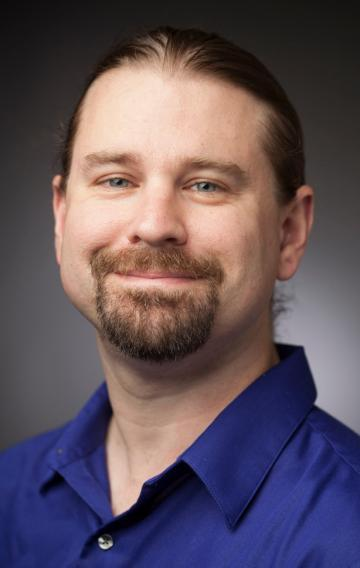
\includegraphics[width=2cm]{media/ross.jpg}};
				\node[anchor=east, minimum width=2cm, left=3mm of ross] {``Wait! Go talk to Matt Mason!''};
			\end{tikzpicture}
		\end{frame}

		\begin{frame}
			\addtocounter{framenumber}{-1}
			\frametitle{How I Ended Up Here (Some Context) VII}
			\begin{tikzpicture}[overlay, remember picture]
				\node[anchor=south east] (ri-logo) at ($(current page.south east)+(-5mm,10mm)$) {
\includegraphics[width=16mm]{assets/ri-logo.eps}};
				\fontsize{12}{10}
				\node[anchor=south west] (me) at ($(current page.south west)+(5mm,10mm)$) {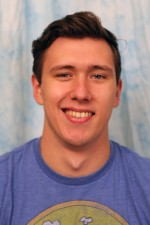
\includegraphics[width=2cm]{media/me.jpg}};
				\node[minimum width=2cm, right=3mm of me] {``(skeptical) Okay...''};
				\node[anchor=north east] (ross) at ($(current page.north east)+(-5mm,-15mm)$) {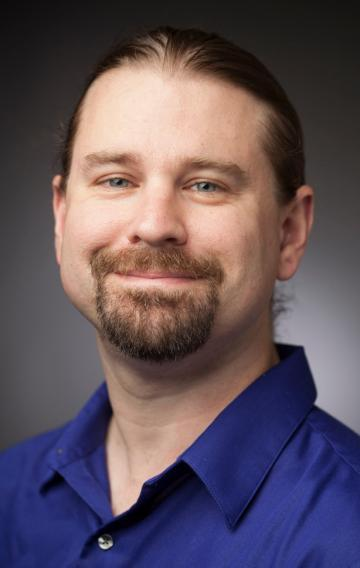
\includegraphics[width=2cm]{media/ross.jpg}};
				\node[anchor=east, minimum width=2cm, left=3mm of ross] {\color{gray}``Wait! Go talk to Matt Mason!''};
			\end{tikzpicture}
		\end{frame}
	
		\begin{frame}
			\addtocounter{framenumber}{-1}
			\frametitle{How I Ended Up Here (Some Context) VIII}
			\begin{tikzpicture}[overlay, remember picture]
				\node[anchor=south east] (ri-logo) at ($(current page.south east)+(-5mm,10mm)$) {
\includegraphics[width=16mm]{assets/ri-logo.eps}};
				\fontsize{12}{15}
				\node[anchor=south west] (me) at ($(current page.south west)+(5mm,10mm)$) {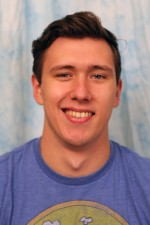
\includegraphics[width=2cm]{media/me.jpg}};
				\node[minimum width=2cm, right=3mm of me] {\color{gray}``(skeptical) Okay...''};
				\node[anchor=north east] (matt) at ($(current page.north east)+(-5mm,-15mm)$) {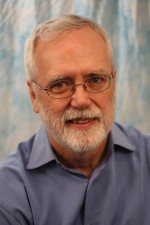
\includegraphics[width=2cm]{media/mason.jpg}};
				\node[anchor=east, text width=5cm, left=3mm of matt, align=right] {``Manipulation is awesome! \\And I have money! \\And I don't micromanage!''};
			\end{tikzpicture}
		\end{frame}
	
		\begin{frame}
			\addtocounter{framenumber}{-1}
			\frametitle{How I Ended Up Here (Some Context) IX}
			\begin{tikzpicture}[overlay, remember picture]
				\node[anchor=south east] (ri-logo) at ($(current page.south east)+(-5mm,10mm)$) {
\includegraphics[width=16mm]{assets/ri-logo.eps}};
				\fontsize{12}{15}
				\node[anchor=south west] (me) at ($(current page.south west)+(5mm,10mm)$) {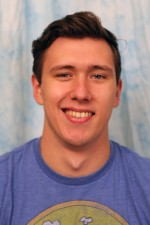
\includegraphics[width=2cm]{media/me.jpg}};
				\node[minimum width=2cm, right=3mm of me] {``(excited) Works for me!''};
				\node[anchor=north east] (matt) at ($(current page.north east)+(-5mm,-15mm)$) {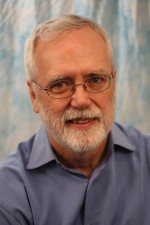
\includegraphics[width=2cm]{media/mason.jpg}};
				\node[anchor=east, text width=5cm, left=3mm of matt, align=right] {\color{gray}``Manipulation is awesome! \\And I have money! \\And I don't micromanage!''};
			\end{tikzpicture}
		\end{frame}
	
		\begin{frame}
			\addtocounter{framenumber}{-1}
			\frametitle{How I Ended Up Here (Some Context) X}
			\begin{tikzpicture}[overlay, remember picture]
				\node[anchor=south east] (ri-logo) at ($(current page.south east)+(-5mm,10mm)$) {
\includegraphics[width=16mm]{assets/ri-logo.eps}};
				\fontsize{12}{15}
				\node[anchor=south west] (me) at ($(current page.south west)+(5mm,10mm)$) {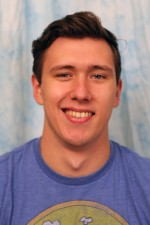
\includegraphics[width=2cm]{media/me.jpg}};
				\node[minimum width=2cm, right=3mm of me] {\color{gray}``(excited) Works for me!''};
				\node[anchor=north east] (matt) at ($(current page.north east)+(-5mm,-15mm)$) {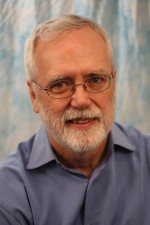
\includegraphics[width=2cm]{media/mason.jpg}};
				\node[anchor=east, minimum width=2cm, left=3mm of matt, align=right] {``Fantastic, go forth and prosper!''};
			\end{tikzpicture}
		\end{frame}

		\begin{frame}
			\addtocounter{framenumber}{-1}
			\frametitle{How I Ended Up Here (Some Context) XI}
			\begin{tikzpicture}[overlay, remember picture]
				\node[anchor=south east] (ri-logo) at ($(current page.south east)+(-5mm,10mm)$) {
\includegraphics[width=16mm]{assets/ri-logo.eps}};
				\fontsize{12}{15}
				\node[anchor=south west] (me) at ($(current page.south west)+(5mm,10mm)$) {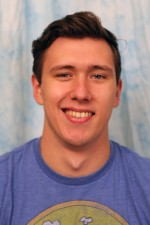
\includegraphics[width=2cm]{media/me.jpg}};
				\node[text width=8cm, right=3mm of me, align=left] {``I've been meaning to read Hogan's famous \emph{Impedance Control}~\autocite{hogan1985impedance} paper, I guess I'll start there...''};
			\end{tikzpicture}
		\end{frame}
	
		\begin{frame}
			\addtocounter{framenumber}{-1}
			\frametitle{How I Ended Up Here (Some Context) XII}
			\begin{tikzpicture}[overlay, remember picture]
				\fontsize{18}{15}
				\node[anchor=center, minimum width=2cm] at (current page.center) {\dots~Two Years Later \dots};
			\end{tikzpicture}
		\end{frame}

		\begin{frame}
		\frametitle{Me, circa July 2018}
			\begin{tikzpicture}[overlay, remember picture]
				\node[anchor=center] (paranoid) at (current page.center) {
\includegraphics[width=8cm]{media/charlie-paranoid}};
				\node[anchor=center, below=0mm of paranoid] {``So it's all about causality\dots~and feedback!''};
			\end{tikzpicture}
		\end{frame}
	
	\section{The Big Picture}
		\begin{frame}
			\frametitle{Back to Basics}
			\begin{itemize}[<+->]
				\item Want a concise \emph{theory of robotics}\dots
				\item Interested in the \emph{physics} common to robotics problems
				\item Not worried about SLAM, POMDPs, etc\dots~there are bigger fish to fry (we're skimming over the basics!)
					\begin{itemize}
						\item i.e. Moravec's paradox \autocite{moravec1988mind}
					\end{itemize}
				\item Inherently a \emph{breadth-first} approach, since we're looking for a unifying framework
			\end{itemize}
		\end{frame}
	
		\begin{frame}
			\frametitle{Problem 1: What is a Robot?}
			\begin{itemize}
				\item I know it's a cliché to bring this up\dots \pause~but I must! \pause
				\begin{itemize}
					\item Does the ambiguity really matter? \pause
					\item Maybe not, but some unifying \emph{theme} would be useful!
				\end{itemize}
			\end{itemize}
		\end{frame}
	
		\begin{frame}
			\frametitle{Problem 2: What is Manipulation?}
			\begin{itemize}
				\item To be honest, I had a very shallow understanding of manipulation until I met Matt \pause
					\begin{itemize}
						\item I imagined it was just factory robot stuff \pause
						\item It took some reflection to appreciate the depth of ``manipulation''
					\end{itemize}
			\end{itemize}
		\end{frame}
	
		\begin{frame}
			\frametitle{Problem 2: What is Manipulation?}
			\begin{tikzpicture}[overlay, remember picture]
				\fontsize{15}{12}
				\node[anchor=center, text width=0.8\textwidth,align=center] (manip-def) at ($(current page.center)+(0,-3mm)$) {``Manipulation refers to an agent’s control of its environment through selective contact.''};
				\small
				\node[anchor=south east, align=right] at ($(current page.south east)+(-1cm,1cm)$) {--- \emph{Matt Mason}, ``Toward Robotic Manipulation'' \autocite{Mason2018}};
			\end{tikzpicture}
		\end{frame}
	
		\begin{frame}
			\frametitle{Problem 3: Locomotion and Manipulation, Segregated}
			\begin{itemize}
				\item Locomotion and manipulation are studied separately in robotics\pause
					\begin{itemize}
						\item \dots~and biomechanics, for that matter
						\item Seems quite natural at first, we all talk about the two as separate specializations in robotics
					\end{itemize}\pause
				\item Eventually, the notion of \emph{``duality''} comes up\dots
				\begin{itemize}\pause
					\item Locomotion and manipulation sometimes overlap
						\begin{itemize}
							\item Pai et al.'s \emph{Platonic Beasts} \autocite{pai1994platonic}
							\item Mason et al.'s \emph{Mobipulator} \autocite{MasonMobileManipulator1999} \autocite{MasonDesktopMobileManipulators2000}
							\item Also, literally everywhere in biology
						\end{itemize}
					\item Perhaps it just comes down to a change of reference?
						\begin{itemize}
							\item Just a matter of ``what pushes off of what?''
							\item Locomotion is ``self-manipulation'', e.g. Aaron Johnson's PhD thesis \autocite{johnson2014self} and related works \autocite{johnson2012standing}\autocite{johnson2016hybrid}
						\end{itemize}
				\end{itemize}
			\end{itemize}
		\end{frame}
	
		\begin{frame}
			\frametitle{Problem 3: Locomotion and Manipulation, United}
			\vspace{-6em}
			\begin{itemize}
				\item The ``self-manipulation'' view of locomotion is consistent with our definition of ``manipulation'':
					\begin{itemize}
						\item An agent may control its environment through selective contact (i.e. ``manipulation'') by moving about in it (i.e. ``locomotion''). \footnotemark
					\end{itemize}
			\end{itemize}
			\footnotetext{It helps to take on an egocentric point of view to visualize this.}
			\pause
			\begin{tikzpicture}[overlay, remember picture]
				\fontsize{15}{12}
				\node[anchor=center,text width=0.8\textwidth,align=center] (loco-manip) at ($(current page.center)+(0,-10mm)$) {So locomotion is just a subset of manipulation!};
			\end{tikzpicture}
		\end{frame}
	
		\begin{frame}
			\frametitle{Problem 3: Locomotion and Manipulation, United}
			\begin{itemize}
				\item Not a terribly practical insight\dots \pause~but thinking back to \emph{Problem 1}\dots
			\end{itemize}
			\begin{tikzpicture}[overlay, remember picture]
				\node[anchor=center,text width=0.8\textwidth,align=center] (manip-is-king) at ($(current page.center)+(0,-10mm)$) {\Large \color{red} Manipulation \emph{is} the central theme in robotics!};
			\end{tikzpicture}
		\end{frame}
	
		\begin{frame}
			\frametitle{Embodiment \& Hogan's Physical-Equivalence ``Postulate''}
			\begin{itemize}[<+->]
				\item Embodiment
					\begin{itemize}
						\item Vaguely, the idea that robots exist in the real world and are inherently tied to their environment
						\item Presently resides in the cognitive science community (as in ``embodied \emph{cognition}'')
					\end{itemize}
				\item \emph{Hogan's} Physical-Equivalent Principle
					\begin{itemize}
						\item ``It is impossible tO devise a controller which will cause a physical system to present an apparent behavior 10 its environment which is distinguishable from that of a purely physical system'' \autocite{hogan1985impedance}
						\item Basic argument for this is ``you can't break thermodynamic laws''
						\item But more intuitively, the robot is a real thing, you can't make it do not real things
					\end{itemize}
			\end{itemize}
		\end{frame}
	
	\section{A Unifying Framework}
		\begin{frame}
			\frametitle{Port-Hamiltonian Systems Theory}
			\begin{itemize}[<+->]
				\item The symbiosis of:
					\begin{itemize}[<+->]
						\item Bond graph theory (\emph{Paynter, Hogan, Breedveld, van Dijk})
						\item Hamiltonian dynamics on manifolds (i.e. ``geometric mechanics'')
						\item Poisson / Dirac structures
					\end{itemize}
				\item Principal contributors include \emph{Stramigioli, van der Schaft, Maschke}
			\end{itemize}
		\end{frame}
	
		\begin{frame}
			\frametitle{Port-Hamiltonian Systems Theory}
			\begin{itemize}
				\item Port-based Analysis
					\begin{itemize}
						\item Inherits the bond-graph notion of power ports
						\item Treats systems in terms of power flow between components
						\item Each bond represents the conjugate pair of an effort and flow
					\end{itemize}
			\end{itemize}
		\end{frame}
	
		\begin{frame}
			\frametitle{Port-Hamiltonian Systems Theory}
			\begin{itemize}
				\item Hamiltonian Dynamics
					\begin{itemize}
						\item Provides a fully geometric (intrinsic, coordinate free) description of system dynamics
						\item Equivalent to (and convertible from/to) Lagrangian formulation, but better!
							\begin{itemize} 
								\item Riemannian geometry of Lagrangian dynamics replaced with symplectic geometry, in which fundamental invariants are preserved
								\item Configuration space of Lagrangian dynamics replaced with state space
								\item Hamiltonian formulation directly yields a system of first order differential equations
							\end{itemize}
						\item Avoiding nonholonomic constraints yields explicit ODE\footnote{May be a stiff explicit ODE! So, soften your intermittent contacts!}
					\end{itemize}
			\end{itemize}
		\end{frame}
	
	
	
		\begin{frame}
			\frametitle{Port-Hamiltonian Systems Theory}
			\begin{itemize}
				\item System fully defined by: 
					\begin{itemize}
						\item Energy function captures all energy storage elements in system
						\item Resistive structure captures all dissipative elements in system
						\item Poisson or Dirac interconnection structure defines power flow within system
							\begin{itemize}
								\item \emph{Storage port} connects to energy storage
								\item \emph{Dissipative port} connects to resistive structure
								\item \emph{Interaction port} connects to environment (\textbf{dynamic system} not known a-priori or directly controlled)
								\item \emph{Controller port} connects to controller (\textbf{dynamic system} that the designer has control over)
							\end{itemize}
					\end{itemize}
			\end{itemize}
		\end{frame}
	
		\begin{frame}
			\frametitle{Working Through an Example}
		\end{frame}
	
	\section{Closing Thoughts}
		\begin{frame}
			\frametitle{Closing Thoughts}
			\begin{itemize}
				\item Manipulation is the common theme in robotics
				\item Embodiment \Leftrightarrow Hogan's Physical Equivalence Principle \autocite{hogan1985impedance}
				\item Port-Hamiltonian Systems Theory is the framework to unify robotics
			\end{itemize}
		\end{frame}
		
%%%%%%%%%%%%%%%%%%%%%%%%%%%%%%%%%%%%%%%%%
	\setcounter{showProgressBar}{0}
	\setcounter{showSlideNumbers}{0}
	
	\appendix
	\backupbegin
	
	\section{Acknowledgments}
	
%		\begin{frame}
%	\frametitle{Teaching with CMU's Gelfand Outreach Center}
%	\begin{tikzpicture}[overlay, remember picture]
%	\node[anchor=south east] (gelfand-logo) at ($(current page.south east) + (-8mm, 8mm)$) {
\includegraphics[width=4cm]{media/gelfand-logo.jpg}};
%	\end{tikzpicture}
%	\vspace{9em}
%	\begin{itemize}
%		\item Introduction to Robotics with the Finch Platform
%		\begin{itemize}
%			\item Each session is 5 days, 3 hrs/day
%			\item 4\textsuperscript{th} and 5\textsuperscript{th} graders
%			\item 1 session Summer 2017 + 2 sessions Summer 2018
%		\end{itemize}
%	\end{itemize}
%\end{frame}
%
%\begin{frame}
%\frametitle{Teaching with CMU's Gelfand Outreach Center}
%\begin{tikzpicture}[overlay, remember picture]
%\node[anchor=south east] (gelfand-logo) at ($(current page.south east) + (-8mm, 8mm)$) {
\includegraphics[width=4cm]{media/gelfand-logo.jpg}};
%\end{tikzpicture}
%\vspace{9em}
%\begin{itemize}
%\item Saturday Series LEGO WeDo Robotics
%\begin{itemize}
%	\item 3 hour course
%	\item 2\textsuperscript{nd} and 3\textsuperscript{rd} graders
%	\item 1 session Spring 2018
%\end{itemize}
%\end{itemize}
%\end{frame}
%
%\begin{frame}
%\frametitle{Robotics Institute Meme Facebook Page}
%\begin{tikzpicture}[overlay, remember picture]
%\node[anchor=center] (ri-meme-screenshot) at (current page.center) {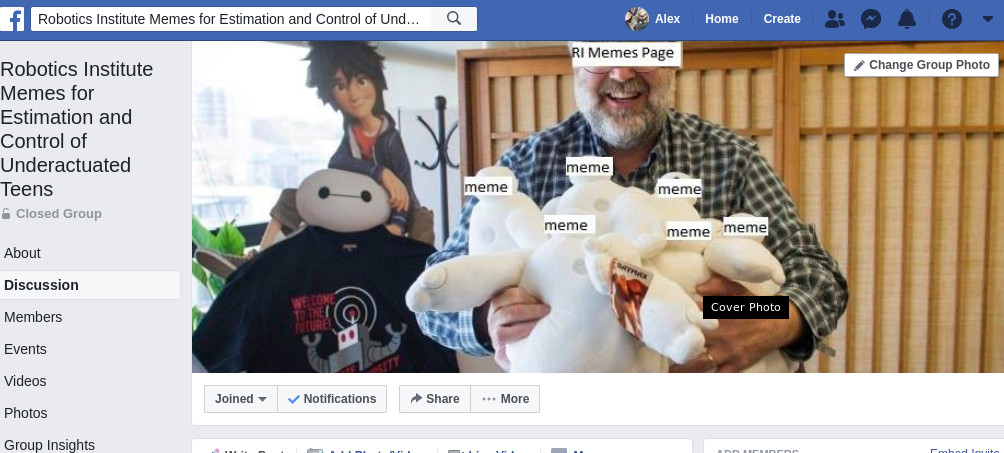
\includegraphics[width=\textwidth]{media/ri-memes.jpg}};
%\end{tikzpicture}
%\end{frame}
%
%\begin{frame}
%\frametitle{Robotics Institute Meme Facebook Page}
%\vspace{9em}
%\begin{itemize}
%\item Some statistics:
%\begin{itemize}
%\item The RI's first and only meme page
%\item Formed in March 2018
%\item 170 members
%\item 30 memes, 23 original contributions!
%\end{itemize}
%\end{itemize}
%\begin{tikzpicture}[overlay, remember picture]
%\node[anchor=south east] (ri-meme-3) at ($(current page.south east) + (2mm,5mm)$) {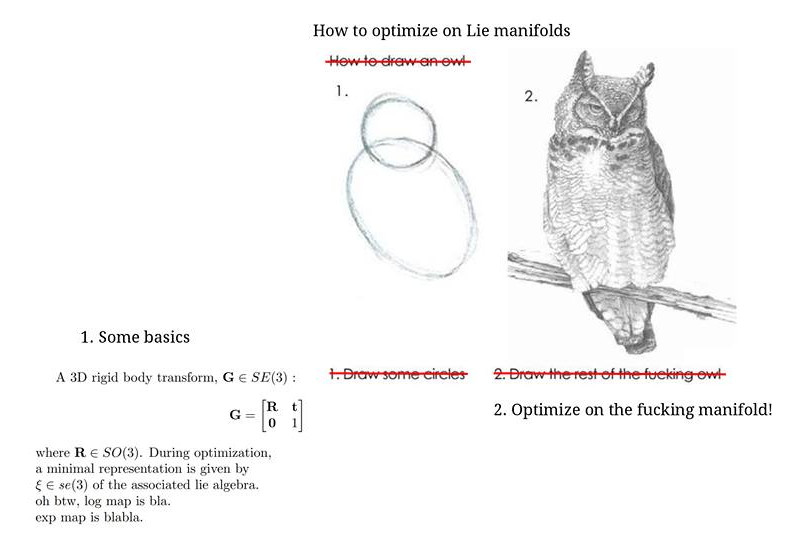
\includegraphics[width=7.5cm]{media/ri-meme-manifold-optimization.jpg}};
%\end{tikzpicture}
%\begin{tikzpicture}[overlay, remember picture]
%\node[anchor=north east] (ri-meme-1) at ($(current page.north east) + (-45mm,-12mm)$) {
\includegraphics[width=3.5cm]{media/ri-meme-thesis-anxiety.jpg}};
%\end{tikzpicture}
%\begin{tikzpicture}[overlay, remember picture]
%\node[anchor=north west] (ri-meme-2) at ($(current page.north west) + (10mm,-12mm)$) {
\includegraphics[width=5cm]{media/ri-meme-ros-sleep.jpg}};
%\end{tikzpicture}
%\end{frame}
	
	\begin{frame}
	\frametitle{Cheers}
		\begin{itemize}
			\item Matt Mason
			\item Aaron Johnson \& Will Martin
			\item The MLab
			\item Ross Knepper, Hod Lipson, Ephrahim Garcia, Boris Kogan, Mike Meller
			\item Jean Harpley
			\item Cameron
			\item Malcolm X, Nina Simone, and George Harrison
			\item Parents
		\end{itemize}
	\end{frame}

	\section{Questions?}
	
	\section{Bibliography}
	\nocite{*}
	\begin{frame}[allowframebreaks]
		\frametitle{Bibliography}
		\printbibliography[heading=none]
	\end{frame}

	\backupend

\end{document}
